\chapter{Kappa: a simplified parallel logic processing primitive}
\label{kappa}

This chapter gives an analysis of the implementation of the
breadth-first partitioning scheduling strategy without using
oracles.  The oracle-based strategy used in PrologPF is compared with a
simplified technique using a special proposition \texttt{kappa}.

A novel parallel processing primitive \texttt{kappa}
is described, suitable for use
with any standard Prolog.  The technique is similar to the breadth-first
partitioning strategy of PrologPF but can be implemented without the
use of oracles \cite{CA87}.  The limitations of the new primitive
are compared with the strategy improvements available to PrologPF through
the improved exploitation of oracles.

%%%%%%%%%%%%%%%%%%%%%%
\section{Background} %
%%%%%%%%%%%%%%%%%%%%%%

Chapter \ref{bfp_depth} reviews in detail the breadth-first
partitioning strategy using oracles to define the root of each
subtree to be allocated to an available path processor.

In the first phase of execution, the search is bounded by a
selected depth limit $L$.  The open branches found at this limit
are recorded as a number $S$ of \textit{oracles}, each representing the
sequence of clauses used to arrive at the point in the search at which
the depth limit was reached.  An \textit{oracle stack} is used to
accumulate the open oracles during this first oracle discovery phase.
While the search in the initial phase is bounded by $L$,
the standard Prolog depth-first left-to-right search is used, and
the $S$ open oracles form an ordered list in the order
of discovery.  Figure \ref{kappa_bfp} shows an example subtree traversed
during the depth-limited initial phase, with the resultant oracle
stack as a data structure representing the paths in the reduced tree.

\begin{figure}[htbp]
\vspace{5mm} \hbox to \hsize{\hfill \psfig{file={kappa/ps/kappa_bfp.ps}} \hfill}
\caption{Use of oracles in breadth-first partitioning.}
\vspace{5mm}
\label{kappa_bfp}
\end{figure}

The oracles in the oracle stack can be allocated to a number of
\textit{path processors} whose role is to follow each assigned oracle
to recreate the environment required at the root of the associated
subtree, and then to continue the search of that subtree.

The \textit{breadth-first partitioning strategy} used by PrologPF proceeds
in the two phases of oracle discovery and subsequent subtree search.
While the model supports the use of a single control processor for
the execution of the first phase and then the allocation 
and communication of the oracles,
a distributed model is used in PrologPF in which all the path
processors execute the first phase and create a local copy of the
oracle stack.  The path processors then use the parameters $G$ and
$N$ representing the processor group size and the unique processor
number respectively to select disjoint subsets of oracles from the oracle stack.

%%%%%%%%%%%%%%%%%%%%%%%%%%%%%%%%%%%%%%%%%%%%%%%%%%%%%%
\section{Breadth-first partitioning without oracles} %
%%%%%%%%%%%%%%%%%%%%%%%%%%%%%%%%%%%%%%%%%%%%%%%%%%%%%%
\label{no_orcs}

If the two phases of the breadth-first partitioning algorithm are
interleaved, it is possible to create a similar scheduling strategy
without the use of oracles.  PrologPF completes the first oracle
discovery phase before assigning the open oracles to the available
path processors.  In practice the oracle assignment function is fixed
before the start of execution, such that the assignment can be
performed independently on each path processor.  However, with 
reference to Figure \ref{kappa_bfp}, on discovery of the first open
oracle at the depth limit L the Prolog stacks and heap contain the environment
necessary for the continued search of the subtree labelled A in the
figure.  This is the environment recreated when the oracle is followed
during the second phase of BFP.  With a suitable filtering function
applied at the depth limit L, the subtrees can be selected and searched
by the path processors \textit{as the open branches at L are discovered}.
The principles of this strategy without oracles are as follows:
\begin{itemize}
\item{The phases equivalent to the initial oracle discovery and 
  subsequent subtree search in PrologPF are interleaved.}
\item{Execution proceeds without maintenance of the current oracle,
  instead exploiting the environment constructed during the
  search beneath the depth limit.}
\item{Each path processor executes the search from the root of the
  search tree, with the following assigned parameters:
  \begin{description}
  \item[$G$: ]{The number of path processors in the group.}
  \item[$N$: ]{The unique processor number of the given path processor.}
  \item[$L$: ]{The selected depth limit.}
  \end{description}}
\item{The search is generally limited to the depth set by $L$, with a count
  accumulating the number of times this depth limit is reached during
  the depth-first left-to-right search.  This count is equivalent to the
  oracle number in the ordered stack resulting from the first phase of
  BFP.  The point in the search tree at which an open branch is discovered at
  the depth limit $L$ is called a \textit{port}.
  Each time the count is incremented, the selection function is
  applied to determine whether the search should continue with the subtree
  beneath the port, or whether the port should be skipped.}
\item{A suitable selection function will ensure that all ports are selected
  by the combined group of path processors, and no port is selected 
  more than once.  As with the BFP algorithm in PrologPF, a good selection
  function would allocate the work beneath the ports evenly.  In the
  absence of a work estimation function, an equal number of
  ports can be allocated to
  each path processor.}
\end{itemize}

Figure \ref{port_tree} shows a search tree during the execution of
a scheduling strategy similar to BFP without using oracles.  The ports
are identified at the depth limit L,  and the selection function at a
given path processor is illustrated.

\begin{figure}[htbp]
\vspace{5mm} \hbox to \hsize{\hfill \psfig{file={kappa/ps/port_tree.ps}} \hfill}
\caption{Search tree partitioning without oracles.}
\vspace{5mm}
\label{port_tree}
\end{figure}

The path processor executes the search bounded by the depth limit until
a port is accepted by the selection function, at which point the search
continues with the subtree beneath that port.  On completion of that
subtree,  the search continues bounded by the depth limit and the
selection function.

%%%%%%%%%%%%%%%%%%%%%%%%%%%%%%%%%%%%%%%%%%%%%%%%%%%
\section{The gate proposition \texttt{k\_{}gate}} %
%%%%%%%%%%%%%%%%%%%%%%%%%%%%%%%%%%%%%%%%%%%%%%%%%%%

The selection function described in Section \ref{no_orcs} 
can be represented by a proposition tested each time
a subgoal is called or executed.  If the current depth is not that of the
depth limit, then the proposition succeeds.  If the depth limit has been
reached, then the proposition fails unless the current port is assigned
to the given path processor.

One suitable function which will evenly allocate the ports to the
available path processors is:
\centerline{$((\mbox{port\_{}number}-N) \mbox{ mod } G) = 0$}

The selection of the ports \textit{modulo G} means that the path
processors search the subtree beneath every $G$th port, beginning
with the $N$th.  Thus with $G$ path processors, allocated values of
$N$ from 0 to $G-1$, all ports will be uniquely allocated.

A pseudo-Prolog proposition providing the port
selection behaviour using this function is \texttt{k\_{}gate}, given
below:
\begin{verbatim}
k_gate :- current_depth <> L.
k_gate :- current_depth = L, 
          increment port_number, 
          (port_number - N) mod G = 0.
\end{verbatim}

The proposition accesses global values for the current depth, the
assigned depth limit $L$, and \texttt{port\_{}number},
the number of ports found so far.  \texttt{k\_{}gate} has the side-effect
of incrementing \texttt{port\_{}number} each time the depth limit is reached.
\texttt{port\_{}number} is initially 0.

%%%%%%%%%%%%%%%%%%%%%%%%%%
\section{\texttt{kappa}} %
%%%%%%%%%%%%%%%%%%%%%%%%%%

\texttt{kappa} is the proposition representing the parallel partitioning
primitive inserted into the user program.  In the absence of an existing
global system value representing the search depth, \texttt{kappa} can
accumulate a depth value and call \texttt{k\_{}gate} to determine
success or failure.  \texttt{depth} is initially 0.
\begin{verbatim}
kappa :- increment depth, k_gate.
kappa :- decrement depth, fail.
\end{verbatim}
In the example of the \texttt{member/factorial} program given in Section
\ref{bfp_stream_and}
the user code can be modified to use \texttt{kappa} as follows:
\begin{verbatim}
member(X,[X|_]).
member(X,[_|Y]) :- kappa, member(X,Y).

fact(1,1).
fact(N,F) :- kappa, N > 1,
             kappa, N1 is N - 1,
             kappa, fact(N1,F1),
             kappa, F is N * F1.
             
:- kappa, member(X,[4,3,2,1]), kappa, fact(X, F).
\end{verbatim}
Preceding every goal with a call to the proposition \texttt{kappa} can
be achieved automatically through the use of the utility relation
\texttt{term\_{}expansion/2} provided with many Prolog implementations
\cite{BBP+94}.  If \texttt{kappa} is only used at selected positions
in the program, then similar behaviour is achieved with a new
meaning for the \textit{depth} value used in the selection 
algorithm.  In this case, the depth value is taken to mean the depth
of the calls to \texttt{kappa}, which is no longer equal to the
current depth in the and-or search tree.

Many implementations of Prolog provide a mechanism to incorporate C
code into procedure definitions.  This capability permits efficient
implementation of the \texttt{kappa} primitive, integrating the
function of \texttt{k\_{}gate}, resulting in the final definition
of \texttt{kappa} given in Table \ref{kappa_code}.

\begin{table}[htbp]
{\small
\begin{tabular}{| l l l |}
\hline
& & \\
\verb?kappa? & \verb?:-? & \verb?if ((++depth == L) && ((++port_number - N) mod G == 0))? \\
 & & \verb?then succeed? \\
 & & \verb?else fail.? \\
\verb?kappa? & \verb?:-?  & \verb?--depth, fail.?\\
 & & \\
\hline
\end{tabular}
}
\caption{Definition of parallelisation primitive \texttt{kappa}.}
\label{kappa_code}
\end{table}


%%%%%%%%%%%%%%%%%%%%%%%%%%%%%%%%%%%%%%%%%%%%%%%%%%%%%%%
\section{Kappa at every subgoal versus selective use} %
%%%%%%%%%%%%%%%%%%%%%%%%%%%%%%%%%%%%%%%%%%%%%%%%%%%%%%%

If the special proposition \texttt{kappa} is inserted before every subgoal in
the user program, the global depth value updated by the frequent calls to
\texttt{kappa} is equal to the current depth of the search into the and-or
tree of the original program.  With the example of the \texttt{member/factorial}
example program given in
Chapter \ref{bfp_depth}, Figure \ref{stream_and}, the selection function provided by
\texttt{kappa} can be viewed as a horizontal boundary with ports at a constant
and-or depth.  The situation is illustrated in Figure \ref{horiz_ports}

\begin{figure}[htbp]
\vspace{5mm} \hbox to \hsize{\hfill \psfig{file={kappa/ps/horiz_ports.ps}} \hfill}
\caption{Search tree for \texttt{member/fact} program with horizontal selection function.}
\vspace{5mm}
\label{horiz_ports}
\end{figure}

However, \texttt{kappa} can be more selectively added to a user program for
similar benefits without the overhead of a call to the proposition before
every original subgoal.  An example of the selective use of \texttt{kappa}
in the \texttt{member/factorial} program is:
\begin{verbatim}
member(X,[X|_]).
member(X,[_|Y]) :- member(X,Y).

fact(1,1).
fact(N,F) :- N > 1,
             N1 is N - 1,
             kappa, fact(N1,F1),
             F is N * F1.
             
:- member(X,[4,3,2,1]), kappa, fact(X, F).
\end{verbatim}
In the example above, only the \texttt{fact} relation is associated with
the \texttt{kappa} proposition.  The depth value maintained by \texttt{kappa}
is now purely the depth into the \texttt{fact} relation, and a diagram
representing the search tree is given in Figure \ref{sloping_ports}.

\begin{figure}[htbp]
\vspace{5mm} \hbox to \hsize{\hfill \psfig{file={kappa/ps/sloping_ports.ps}} \hfill}
\caption{Search tree for \texttt{member/fact} program with sloping selection function.}
\vspace{5mm}
\label{sloping_ports}
\end{figure}

With selective use of \texttt{kappa}, the programmer (or compiler) would select those
relations known to generate a large number of branches near the root of the search
tree.  In the minimal case, \texttt{kappa} might be associated with just one relation in
the user program, and an appropriately small value of the depth limit would be used.
The \texttt{member/fact} program given above will partition the work satisfactorily with
\texttt{kappa} associated with the relation \texttt{fact} and a depth limit set at 1.
Higher values of the depth limit $L$ will not improve the partitioning of the problem
as the \texttt{fact} relation is deterministic and partitioning deeper into the
\texttt{fact} relation will result in the same number of ports.

A more general example of the selective use of \texttt{kappa} is given in the
procedure \texttt{findsum} below
\footnote{\texttt{select(L,X,L1)} is a library relation with X a value from list L
  with the remainder of the list in L1}. 
\begin{verbatim}
% findsum(List_in, Sum, List_out): List_out is list of integers from
%                                  List_in which sum to value in Sum

findsum(L,S,[X|Y]) :- select(L,X,L1), S1 is S - X, kappa, findsum(L1,S1,Y). 
findsum(_,0,[]).

:- findsum([1,2,3,5,7,11],14, X).
\end{verbatim}
If the depth limit $L$ for the execution of the problem is set at 1, then partitioning will
take place after selection of the first candidate integer for the sum.  For $L=2$,
partitioning will take place after the selection of two integers, and so on.

%%%%%%%%%%%%%%%%%%%%%%%%%%%%%%%%%%%%%
\section{Efficiency considerations} %
%%%%%%%%%%%%%%%%%%%%%%%%%%%%%%%%%%%%%

\subsection{Sequential computation when $\mbox{depth}<L$}
%%%%%%%%%%%%

PrologPF performs the initial pseudo-breadth-first search without advantage from
the parallel processing available in the distributed system.  Two techniques are
available to PrologPF:
\begin{enumerate}
\item{Perform the initial search in the control processor, and communicate the
  discovered oracles to the available path processors.}
\item{Duplicate the initial search in every path processor, such that an oracle
  stack is held locally on every machine.  The oracles can be allocated using a
  common algorithm ensuring each oracle is allocated to one path processor, and
  all oracles are allocated.}
\end{enumerate}
The implementation used as the subject of this dissertion uses the second
technique, but has been tested with the first.  The earlier implementation
using oracles, DelphiKS \cite{Kle91, Sar95}, also used both techniques.

The parallel speedup available with the use of \texttt{kappa} is similarly
limited by the sequential search of the tree beneath the depth limit $L$.
However, the use of \texttt{kappa} requires that the second technique listed
above be used.  The interleaving of the depth-limited search with the 
subsequent subtree search and the lack of oracles means that each path processor
must proceed with the pseudo-depth-first search to create the environment
required at each port before searching an assigned subtree.

The duplicated processing (or equally the sequential processing of the first
technique) imposes a limit on the maximum speedup of the problem.  For PrologPF
this issue is discussed in Chapter \ref{bfp_depth}, Section \ref{orc_discovery}.
If the depth limit is set too large, then a large proportion of the total
search tree may reside within the depth limit $L$, while only the subtrees
at depths greater than $L$ are available for parallel search.

\subsection{Optimal selection of depth limit $L$}
%%%%%%%%%%%%

As with the breadth-first partitioning strategy used by PrologPF, the depth
limit $L$ determines the amount of computation done in the initial sequential
phase of execution, and the number of open branches found.

An optimal value of the depth limit will minimise the amount of recomputation
performed beneath the depth limit while discovering enough ports to provide sufficiently
fine granularity of work in the subtrees to balance the assigned workloads.

The related issue with the BFP strategy is discussed in detail in Chapter \ref{bfp_depth},
Section \ref{bfp_issues}.  The use of \texttt{kappa} avoids the requirement for
oracles by interleaving the subtree search with the pseudo-breadth-first search phase.
Potential optimisations using knowledge of the overall count or distribution of ports
are not available with the use of \texttt{kappa}.

For some small values of the depth limit $L$,  only a small number of ports will
be discovered, perhaps smaller than the number of available path processors.  In
this situation the number of ports present at $L$ will place an upper bound on the
possible speedup.  As with the breadth-first partitioning strategy, an improvement
in speedup may be obtained by iterating through several increasing values of $L$
until the number of ports discovered is at least some multiple of the number of
available path processors.

An executable binary compiled using either PrologPF or with the \texttt{kappa}
primitive can report the number of open oracles or ports found without further
search if:\\
\begin{enumerate}
\item{The program reports the number of open oracles or ports found on completion.}
\item{The program is assigned a unique processor number higher than the maximum
  open oracle or port count.  The modulo arithmetic function used to select would
  in this case assign no ports or oracles to the selected path processor.}
\end{enumerate}
This technique suggests that optimising the number of open oracles or
ports found $S$ provides an estimate for a reasonable value of the depth
limit $L$.

\subsection{Oracle data structures imply limit on $L$}
%%%%%%%%%%%%

PrologPF proceeds in two phases, building the \textit{oracle stack} during the
initial oracle discovery phase.  For a given depth threshold $L$ a number $S$ of
open oracles will be found, to be recorded in the oracle stack.  PrologPF represents
an oracle with a list of integers stored in an array, and the oracle stack is a
two-dimensional array.  The earlier implementation of DelphiKS used the number of
clauses in each procedure to compress the clause index into a binary number of
a variable number of bits \cite{Kle91}.  A tree representation would also be
more compact than the PrologPF arrays.

The storage of the oracles during the first phase of execution in PrologPF imposes
a limit on the number of oracles that can be utilised.  This places constraints on
the acceptable values for the depth limit $L$.  Figure \ref{pent_orc_count} shows the
increase in the number of open oracles discovered by PrologPF at increasing depth
limits.

\begin{figure}[htbp]
\vspace{5mm} \hbox to \hsize{\hfill \psfig{file={kappa/ps/pent_orc_count.ps}} \hfill}
\caption{Count of open oracles for Pentominoes problem for $L=3\ldots 33$.}
\vspace{5mm}
\label{pent_orc_count}
\end{figure}

The oracles recorded on the oracle stack will each have a length equal to the selected
depth limit.  The oracle stack storage requirements for the Pentominoes program are
given in the graph of Figure \ref{pent_orc_storage}.

\begin{figure}[htbp]
\vspace{5mm} \hbox to \hsize{\hfill \psfig{file={kappa/ps/pent_orc_storage.ps}} \hfill}
\caption{Oracle stack size for Pentominoes problem for $L=3\ldots 33$.}
\vspace{5mm}
\label{pent_orc_storage}
\end{figure}

While the storage requirement of the oracle stack imposes a limit on the possible values
of $L$, the use of the parallelisation primitive \texttt{kappa} has no accumulated oracle
information as the execution proceeds.  Thus the use of \texttt{kappa} is more tolerant of
large values of $L$. 

\subsection{Total \texttt{kappa} port count versus PrologPF open oracle count}
%%%%%%%%%%%%

The oracle-based partitioning algorithm used by PrologPF discovers all the open
oracles at the selected depth limit \textit{before} the assignment of the associated
subtrees for search by the available path processors.  As a minimum, the count
$S$ of open oracles is known before the allocation.

While PrologPF takes no advantage of this information in its simple fixed allocation
algorithm, the information may be useful for future improvements.

The simple use of \texttt{kappa} searches each discovered subtree as execution proceeds
in one phase, such that the total port count (equivalent to the PrologPF open oracle
count) cannot be known as a given subtree is searched.

If the total port count is deemed essential for a worthwhile improvement in the
port selection algorithm then the execution of a program using \texttt{kappa} can
proceed in two phases.  The first phase would be completely limited to the
selected depth limit (i.e. the gating proposition would be \texttt{false}.  This
phase would return the number of ports found, and the count or other information made
available to the port selection function as execution proceeds as before.  This
technique would double the overhead of the sequential component of the program
execution.  The times taken for execution of the sequential component of the
Pentominoes problem for the range of depth limits used in Figure \ref{pent_orc_count}
are given in Figure \ref{pent_bf_times}.

\begin{figure}[htbp]
\vspace{5mm} \hbox to \hsize{\hfill \psfig{file={kappa/ps/pent_bf_times.ps}} \hfill}
\caption{Sequential execution component of Pentominoes problem for $L=3\ldots 33$.}
\vspace{5mm}
\label{pent_bf_times}
\end{figure}

The single-cpu execution time of the Pentominoes problem is 445 seconds, so the
sequential execution time is reasonable, particularly for systems with few available
path processors.

\subsection{Work reassignment on path processor failure}
%%%%%%%%%%%%

In the event of path processor failure using PrologPF,
the work can be passed to an alternative
path processor by redistributing the affected oracles.  The newly assigned path
processors can efficiently recreate the environment needed at each subtree to
repeat the search of the failed processor.

The impact of a failed processor may be greater with the simple use of the
\texttt{kappa} primitive, as the reconstruction of the environment at a given
\textit{port} requires the complete search of the depth-limited subtree to
the left of that port.  This is because the port number is obtained from a
count of the number of times the selected depth limit has been reached in
the search so far, and the search is strictly depth-first, left-to-right.

The overhead of the processing required to reconstruct the environment at a given
port is bounded by the sequential execution time of the problem up to the
assigned depth limit.  The sequential execution times for the Pentominoes problem
at various depth limits is given in Figure \ref{pent_bf_times}.

\subsection{Solutions found within the depth limit}
%%%%%%%%%%%%

For problems with multiple solutions distributed at various depths in the
and-or search tree, it is possible to select a depth limit which divides
the solutions into those beneath the depth limit and those in the subtrees
beneath the ports.  The search of the tree beneath the depth limit is repeated by
all the path processors, and solutions in this part of the tree will thus be found
and reported by all the path processors.

If the problem requires that duplicate solutions must be avoided, then the issue
caused by the initial search repeated by all the path processors must be addressed.
One technique to ensure unique solutions is to:
\begin{enumerate}
\item{The path processor tags each solution with the
  \textit{depth} at which that solution was found.}
\item{The control processor can accept solutions tagged with a depth less than
  that of the depth limit only from one path processor.  Solutions returned by
  other path processors with depths less than the depth limit are discarded.}
\end{enumerate}
As the depth limit is known to all the path processors and the control processor,
then a similar technique could be used to ensure that only one path processor
(for example, the path processor assigned the unique processor number 0) would return
solutions below the depth limit to the control processor.

%%%%%%%%%%%%%%%%%%%%%%%%%%%%%%%%%
\section{Repeated partitioning} %
%%%%%%%%%%%%%%%%%%%%%%%%%%%%%%%%%

As with the oracle based breadth-first partitioning used in PrologPF, the use
of \texttt{kappa} can allocate differing workloads to the path processors, such that
some will complete before others and become idle for the remainder of the
computation.  The issue for PrologPF is discussed in detail in Chapter \ref{bfp_depth},
Section \ref{bfp_issues}.

If many path processors have completed and become idle, but one or a few are still
busy, then it may be worthwhile to redistribute the work from the busy processors to
the idle processors.  one mechanism to effect this is the repeated application of a
depth limit within the subtree of a busy processor.  The situation is pictorially
represented in Figure \ref{repeat_kappa}

\begin{figure}[htbp]
\vspace{5mm} \hbox to \hsize{\hfill \psfig{file={kappa/ps/repeat_kappa.ps}} \hfill}
\caption{Repeated use of a depth limit and \texttt{kappa} within a subtree.}
\vspace{5mm}
\label{repeat_kappa}
\end{figure}

If it is assumed that other path processors have completed the search of the 
subtrees beneath ports A, B and D in Figure \ref{repeat_kappa}, then path
processor $N$ assigned to port C is still executing.  With a suitable extension
of the port selection function, the group of path processors can all be
set to search the subtree beneath port C at depth L,
with a new depth limit for \texttt{kappa} of L1.  The usual partitioning can occur at
this new depth limit, such that the work has been assigned to all the previously
idle path processors.

A given port in the search tree is uniquely identified by a list of (depth, port number)
tuples.  If \texttt{kappa} is associated with every relation in the user program, such that
the depth used for partitioning is equal to the search depth in the and-or tree, then
the list of (depth, port number) tuples is identical to the equivalent oracle used by
PrologPF with an assumed depth increment of 1.  In Figure \ref{repeat_kappa} the
sequence [(L,C), (L1,C1)] can be considered a compressed form of the oracle leading to
port C1.

This repeated use of incremental depth limits with \texttt{kappa} is similar to
the approach of \textit{work splitting} discussed in Chapter \ref{bfp_depth},
Section \ref{bfp_work_splitting} for PrologPF.  However, the overhead in following
the list of (depth, port number) tuples is much greater then the efficient traversal
of an equivalent oracle.  For repeated use of depth limits with \texttt{kappa}, the
left-most portion of each subtree at each port in the list must be searched to
discover the selected port at the next depth.  For large balanced problems with a high
degree of or-parallelism and thus a large number of even subtrees at each selected
depth, this overhead may still be acceptable.


%%%%%%%%%%%%%%%%%%%%%%%
\section{Conclusions} %
%%%%%%%%%%%%%%%%%%%%%%%

The fixed-allocation 
breadth-first partitioning algorithm with oracles used by PrologPF can be
implemented without using oracles with a special parallel processing primitive
called \texttt{kappa}.  The efficient implemenation and use of \texttt{kappa} requires
support for user C programming and access to global C values in the Prolog system, but
requires no modifications to the Prolog compiler or runtime system.

The use of \texttt{kappa} facilitates simple breadth-first partitioning of Prolog
programs with similar performance
characteristics and issues as those found with PrologPF.

Enhancements to the scheduling strategy possible through the availability of oracles in
the PrologPF environment are not transferrable to the use of \texttt{kappa}.

%%%%%%%%%%%%%%%%%%%
\section{Summary} %
%%%%%%%%%%%%%%%%%%%

The implementation of the breadth-first partitioning scheduling strategy used by
PrologPF uses oracles to represent the subtrees still to be explored at the open
branches at the selected depth limit.

The BFP strategy proceeds in two distinct phases:
\begin{enumerate}
\item{Oracle discovery, in which an oracle stack is built representing all the
  open branches at the selected depth limit.}
\item{Subtree selection and search, in which path processors are allocated disjoint
  subsets of the open oracles and search the referenced subtrees.}
\end{enumerate}

If these two phases are interleaved, a similar allocation strategy can be obtained
without the use of oracles.  The open oracles discovered in BFP are followed in the
second phase to reconstruct the environment pertinent to the subsequent search of
the dependent subtree.  Without oracles, the environment constructed at the point of
discovery of the open branch at the depth limit can be exploited if the
subtree is searched immediately.  The open branches at the depth limit are called
\textit{ports}, and a masking function similar to the oracle allocation function
is required in each path processor, such that each processor skips over the ports
allocated to other path processors.

The process of maintaining a global depth value and performing a port selection
function has been integrated into a novel primitive called \texttt{kappa}.  Calls
to the special proposition \texttt{kappa} are embedded into the 
conjunctive subgoals of the user program, and
the proposition has the following characteristics:
\begin{enumerate}
\item{At depths other then the selected depth limit, \texttt{kappa} is transparent to
  the logic of the program, that is it always succeeds.}
\item{At the depth limit, \texttt{kappa} will succeed at ports allocated to the local
  path processor, and fail otherwise.}
\end{enumerate}

If the special proposition \texttt{kappa} is inserted before every subgoal in every
clause, then the depth value maintained is the same as the depth into the transformed
problem or-only tree used by PrologPF \cite{Sar95}.  \texttt{kappa} can be used
selectively in te user program, as a minimum associated with just one user relation.
The depth information is then limited to the depth of the nested calls of the
selected relations.

The optimal distributed execution of programs using \texttt{kappa}
is influenced by a number of factors:
\begin{enumerate}
\item{The search of the problem tree at depths less than the selected depth limit is
  repeated in every path processor, and is effectively a sequential component of
  the execution.  The time taken for this sequential component places an upper bound
  on the speedup available.}
\item{As with PrologPF, the simple use of \texttt{kappa} relies upon a reasonable value
  for the depth limit at which partitioning takes place.  A depth limit which is too
  small will not generate sufficient ports to permit an even distribution of the work.
  A depth limit which is too high will cause a high proportion of the available work to
  be executed sequentially, reducing the parallel speedup.}
\item{Unlike PrologPF, the use of \texttt{kappa} imoses no requirements for storage of
  oracle information as the depth-limited search progresses.  In general, the use of
  \texttt{kappa} will accomodate larger values of the depth limit than PrologPF.}
\item{As the subtree search is interleaved with the port discovery process, the port
  allocation algorithm cannot use the knowledge of the total number of ports for any
  potential improvement in the efficiency of allocation.  The equivalent information is
  available to PrologPF on completion of the initial oracle discovery phase.}
\item{The work in the subtree beneath each port may vary widely between different ports
  and between different path processors.
  The use of oracles in PrologPF provide the potential for the
  efficient redistribution of work from a busy processor to idle path processors.
  Redistribution of work with the use of \texttt{kappa} will incur a greater overhead of
  the recomputation of the subtree to the left of the current port.}
\end{enumerate}

While optimisations possible in the future enhancement of PrologPF are not available
with the use of \texttt{kappa},  the special proposition can provide the parallel speedup
benefits of the current implementation of PrologPF.